

\tikzset{every picture/.style={line width=0.75pt}} %set default line width to 0.75pt        

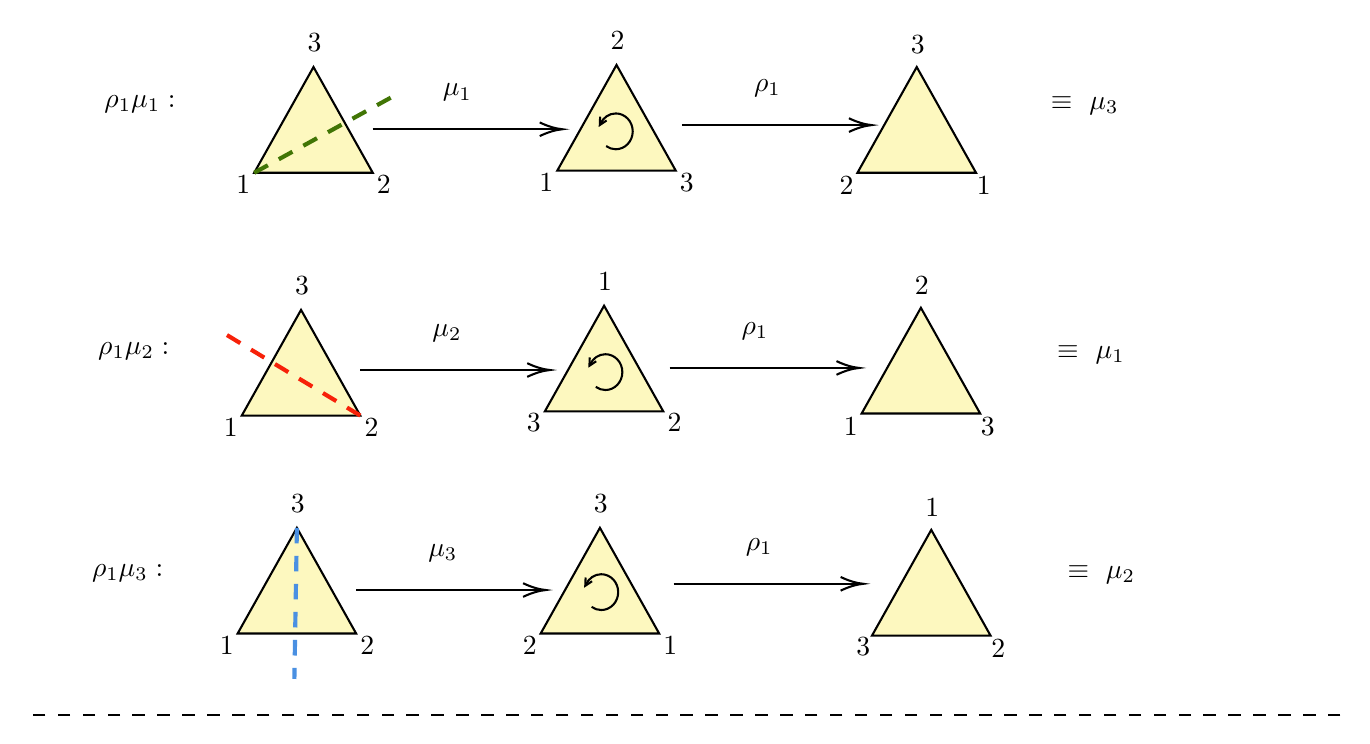
\begin{tikzpicture}[x=0.75pt,y=0.75pt,yscale=-1,xscale=1]
%uncomment if require: \path (0,350); %set diagram left start at 0, and has height of 350

%Shape: Triangle [id:dp19163829570612012] 
\draw  [fill={rgb, 255:red, 250; green, 238; blue, 106 }  ,fill opacity=0.43 ] (281.21,251.75) -- (309.76,302.69) -- (252.65,302.69) -- cycle ;

%Shape: Triangle [id:dp4514811151405802] 
\draw  [fill={rgb, 255:red, 250; green, 238; blue, 106 }  ,fill opacity=0.43 ] (283.21,144.75) -- (311.76,195.69) -- (254.65,195.69) -- cycle ;

%Shape: Triangle [id:dp2789857293750989] 
\draw  [fill={rgb, 255:red, 250; green, 238; blue, 106 }  ,fill opacity=0.43 ] (289.21,28.75) -- (317.76,79.69) -- (260.65,79.69) -- cycle ;

%Shape: Triangle [id:dp046781731174108665] 
\draw  [fill={rgb, 255:red, 250; green, 238; blue, 106 }  ,fill opacity=0.43 ] (435.85,145.75) -- (464.41,196.69) -- (407.29,196.69) -- cycle ;
%Shape: Triangle [id:dp21965592087989438] 
\draw  [fill={rgb, 255:red, 250; green, 238; blue, 106 }  ,fill opacity=0.43 ] (137.21,146.75) -- (165.76,197.69) -- (108.65,197.69) -- cycle ;

%Straight Lines [id:da6171044085428108] 
\draw    (314.75,174.73) -- (404.12,174.73) ;
\draw [shift={(406.12,174.73)}, rotate = 180] [color={rgb, 255:red, 0; green, 0; blue, 0 }  ][line width=0.75]    (10.93,-3.29) .. controls (6.95,-1.4) and (3.31,-0.3) .. (0,0) .. controls (3.31,0.3) and (6.95,1.4) .. (10.93,3.29)   ;
%Shape: Arc [id:dp18073662179695316] 
\draw  [draw opacity=0] (276.49,173.01) .. controls (277.81,170.11) and (280.61,168.11) .. (283.85,168.11) .. controls (288.36,168.11) and (292.01,171.97) .. (292.01,176.74) .. controls (292.01,181.5) and (288.36,185.37) .. (283.85,185.37) .. controls (282.13,185.37) and (280.53,184.8) .. (279.21,183.84) -- (283.85,176.74) -- cycle ; \draw   (276.49,173.01) .. controls (277.81,170.11) and (280.61,168.11) .. (283.85,168.11) .. controls (288.36,168.11) and (292.01,171.97) .. (292.01,176.74) .. controls (292.01,181.5) and (288.36,185.37) .. (283.85,185.37) .. controls (282.13,185.37) and (280.53,184.8) .. (279.21,183.84) ;  
\draw   (279.43,171.51) -- (276.15,173.67) -- (276.31,169.69) ;

%Straight Lines [id:da3068937473833855] 
\draw [color={rgb, 255:red, 247; green, 33; blue, 9 }  ,draw opacity=1 ][line width=1.5]  [dash pattern={on 5.63pt off 4.5pt}]  (165.76,197.69) -- (101,158.58) ;
%Straight Lines [id:da5998407578854817] 
\draw    (165.75,175.73) -- (255.12,175.73) ;
\draw [shift={(257.12,175.73)}, rotate = 180] [color={rgb, 255:red, 0; green, 0; blue, 0 }  ][line width=0.75]    (10.93,-3.29) .. controls (6.95,-1.4) and (3.31,-0.3) .. (0,0) .. controls (3.31,0.3) and (6.95,1.4) .. (10.93,3.29)   ;
%Shape: Triangle [id:dp6236283173447018] 
\draw  [fill={rgb, 255:red, 250; green, 238; blue, 106 }  ,fill opacity=0.43 ] (433.85,29.75) -- (462.41,80.69) -- (405.29,80.69) -- cycle ;
%Shape: Triangle [id:dp9148338393626184] 
\draw  [fill={rgb, 255:red, 250; green, 238; blue, 106 }  ,fill opacity=0.43 ] (143.21,29.75) -- (171.76,80.69) -- (114.65,80.69) -- cycle ;

%Straight Lines [id:da5291595834526982] 
\draw    (320.75,57.73) -- (410.12,57.73) ;
\draw [shift={(412.12,57.73)}, rotate = 180] [color={rgb, 255:red, 0; green, 0; blue, 0 }  ][line width=0.75]    (10.93,-3.29) .. controls (6.95,-1.4) and (3.31,-0.3) .. (0,0) .. controls (3.31,0.3) and (6.95,1.4) .. (10.93,3.29)   ;
%Shape: Arc [id:dp8806276716986381] 
\draw  [draw opacity=0] (281.49,57.01) .. controls (282.81,54.11) and (285.61,52.11) .. (288.85,52.11) .. controls (293.36,52.11) and (297.01,55.97) .. (297.01,60.74) .. controls (297.01,65.5) and (293.36,69.37) .. (288.85,69.37) .. controls (287.13,69.37) and (285.53,68.8) .. (284.21,67.84) -- (288.85,60.74) -- cycle ; \draw   (281.49,57.01) .. controls (282.81,54.11) and (285.61,52.11) .. (288.85,52.11) .. controls (293.36,52.11) and (297.01,55.97) .. (297.01,60.74) .. controls (297.01,65.5) and (293.36,69.37) .. (288.85,69.37) .. controls (287.13,69.37) and (285.53,68.8) .. (284.21,67.84) ;  
\draw   (284.43,55.51) -- (281.15,57.67) -- (281.31,53.69) ;

%Straight Lines [id:da1528001297367797] 
\draw    (171.75,59.73) -- (261.12,59.73) ;
\draw [shift={(263.12,59.73)}, rotate = 180] [color={rgb, 255:red, 0; green, 0; blue, 0 }  ][line width=0.75]    (10.93,-3.29) .. controls (6.95,-1.4) and (3.31,-0.3) .. (0,0) .. controls (3.31,0.3) and (6.95,1.4) .. (10.93,3.29)   ;
%Straight Lines [id:da9454860130046835] 
\draw [color={rgb, 255:red, 65; green, 117; blue, 5 }  ,draw opacity=1 ][line width=1.5]  [dash pattern={on 5.63pt off 4.5pt}]  (114.65,80.69) -- (181,44.2) ;
%Shape: Triangle [id:dp19435915537821324] 
\draw  [fill={rgb, 255:red, 250; green, 238; blue, 106 }  ,fill opacity=0.43 ] (440.85,252.75) -- (469.41,303.69) -- (412.29,303.69) -- cycle ;
%Shape: Triangle [id:dp018841163938158045] 
\draw  [fill={rgb, 255:red, 250; green, 238; blue, 106 }  ,fill opacity=0.43 ] (135.21,251.75) -- (163.76,302.69) -- (106.65,302.69) -- cycle ;

%Straight Lines [id:da43165367131576704] 
\draw    (316.75,278.73) -- (406.12,278.73) ;
\draw [shift={(408.12,278.73)}, rotate = 180] [color={rgb, 255:red, 0; green, 0; blue, 0 }  ][line width=0.75]    (10.93,-3.29) .. controls (6.95,-1.4) and (3.31,-0.3) .. (0,0) .. controls (3.31,0.3) and (6.95,1.4) .. (10.93,3.29)   ;
%Shape: Arc [id:dp469934169778089] 
\draw  [draw opacity=0] (274.49,279.01) .. controls (275.81,276.11) and (278.61,274.11) .. (281.85,274.11) .. controls (286.36,274.11) and (290.01,277.97) .. (290.01,282.74) .. controls (290.01,287.5) and (286.36,291.37) .. (281.85,291.37) .. controls (280.13,291.37) and (278.53,290.8) .. (277.21,289.84) -- (281.85,282.74) -- cycle ; \draw   (274.49,279.01) .. controls (275.81,276.11) and (278.61,274.11) .. (281.85,274.11) .. controls (286.36,274.11) and (290.01,277.97) .. (290.01,282.74) .. controls (290.01,287.5) and (286.36,291.37) .. (281.85,291.37) .. controls (280.13,291.37) and (278.53,290.8) .. (277.21,289.84) ;  
\draw   (277.43,277.51) -- (274.15,279.67) -- (274.31,275.69) ;

%Straight Lines [id:da8338747153912434] 
\draw    (163.75,281.73) -- (253.12,281.73) ;
\draw [shift={(255.12,281.73)}, rotate = 180] [color={rgb, 255:red, 0; green, 0; blue, 0 }  ][line width=0.75]    (10.93,-3.29) .. controls (6.95,-1.4) and (3.31,-0.3) .. (0,0) .. controls (3.31,0.3) and (6.95,1.4) .. (10.93,3.29)   ;
%Straight Lines [id:da4368451154360722] 
\draw [color={rgb, 255:red, 74; green, 144; blue, 226 }  ,draw opacity=1 ][line width=1.5]  [dash pattern={on 5.63pt off 4.5pt}]  (135.21,251.75) -- (134,324.58) ;
%Straight Lines [id:da39602756231413405] 
\draw  [dash pattern={on 4.5pt off 4.5pt}]  (638,341.9) -- (6,341.9) ;

% Text Node
\draw (397.22,197.31) node [anchor=north west][inner sep=0.75pt]    {$1$};
% Text Node
\draw (463.3,197.31) node [anchor=north west][inner sep=0.75pt]    {$3$};
% Text Node
\draw (431.48,129.11) node [anchor=north west][inner sep=0.75pt]    {$2$};
% Text Node
\draw (348,151.4) node [anchor=north west][inner sep=0.75pt]    {$\rho _{1}$};
% Text Node
\draw (199,152.4) node [anchor=north west][inner sep=0.75pt]    {$\mu _{2}$};
% Text Node
\draw (505,268.4) node [anchor=north west][inner sep=0.75pt]    {$\equiv \ \mu _{2}$};
% Text Node
\draw (395.22,81.31) node [anchor=north west][inner sep=0.75pt]    {$2$};
% Text Node
\draw (461.3,81.31) node [anchor=north west][inner sep=0.75pt]    {$1$};
% Text Node
\draw (429.48,13.11) node [anchor=north west][inner sep=0.75pt]    {$3$};
% Text Node
\draw (354,34.4) node [anchor=north west][inner sep=0.75pt]    {$\rho _{1}$};
% Text Node
\draw (204,36.4) node [anchor=north west][inner sep=0.75pt]    {$\mu _{1}$};
% Text Node
\draw (500,162.4) node [anchor=north west][inner sep=0.75pt]    {$\equiv \ \mu _{1}$};
% Text Node
\draw (41,42.12) node [anchor=north west][inner sep=0.75pt]    {$\rho _{1} \mu _{1} :$};
% Text Node
\draw (38,161.12) node [anchor=north west][inner sep=0.75pt]    {$\rho _{1} \mu _{2} :$};
% Text Node
\draw (403.22,303.31) node [anchor=north west][inner sep=0.75pt]    {$3$};
% Text Node
\draw (468.3,304.31) node [anchor=north west][inner sep=0.75pt]    {$2$};
% Text Node
\draw (436.48,236.11) node [anchor=north west][inner sep=0.75pt]    {$1$};
% Text Node
\draw (350,255.4) node [anchor=north west][inner sep=0.75pt]    {$\rho _{1}$};
% Text Node
\draw (197,258.4) node [anchor=north west][inner sep=0.75pt]    {$\mu _{3}$};
% Text Node
\draw (497,42.4) node [anchor=north west][inner sep=0.75pt]    {$\equiv \ \mu _{3}$};
% Text Node
\draw (35,268.12) node [anchor=north west][inner sep=0.75pt]    {$\rho _{1} \mu _{3} :$};
% Text Node
\draw (276.84,234.29) node [anchor=north west][inner sep=0.75pt]    {$3$};
% Text Node
\draw (310.29,302.49) node [anchor=north west][inner sep=0.75pt]    {$1$};
% Text Node
\draw (242.57,302.49) node [anchor=north west][inner sep=0.75pt]    {$2$};
% Text Node
\draw (130.84,234.29) node [anchor=north west][inner sep=0.75pt]    {$3$};
% Text Node
\draw (164.29,302.49) node [anchor=north west][inner sep=0.75pt]    {$2$};
% Text Node
\draw (96.57,302.49) node [anchor=north west][inner sep=0.75pt]    {$1$};
% Text Node
\draw (284.84,11.29) node [anchor=north west][inner sep=0.75pt]    {$2$};
% Text Node
\draw (318.29,79.49) node [anchor=north west][inner sep=0.75pt]    {$3$};
% Text Node
\draw (250.57,79.49) node [anchor=north west][inner sep=0.75pt]    {$1$};
% Text Node
\draw (138.84,12.29) node [anchor=north west][inner sep=0.75pt]    {$3$};
% Text Node
\draw (172.29,80.49) node [anchor=north west][inner sep=0.75pt]    {$2$};
% Text Node
\draw (104.57,80.49) node [anchor=north west][inner sep=0.75pt]    {$1$};
% Text Node
\draw (278.84,127.29) node [anchor=north west][inner sep=0.75pt]    {$1$};
% Text Node
\draw (312.29,195.49) node [anchor=north west][inner sep=0.75pt]    {$2$};
% Text Node
\draw (244.57,195.49) node [anchor=north west][inner sep=0.75pt]    {$3$};
% Text Node
\draw (132.84,129.29) node [anchor=north west][inner sep=0.75pt]    {$3$};
% Text Node
\draw (166.29,197.49) node [anchor=north west][inner sep=0.75pt]    {$2$};
% Text Node
\draw (98.57,197.49) node [anchor=north west][inner sep=0.75pt]    {$1$};


\end{tikzpicture}
